\documentclass[11pt,a4paper]{article}

\usepackage{epsfig}
\usepackage{multicol}

\usepackage[utf8]{inputenc}
\usepackage[brazil]{babel}
\usepackage{fancyheadings}
\usepackage{amsmath}
\usepackage{calrsfs}
\usepackage{enumerate}
\usepackage{enumitem}   
\DeclareGraphicsExtensions{.png,.pdf}
\usepackage{amsmath, amsfonts, amssymb}
\usepackage{esint}
\usepackage{graphicx}
\usepackage{multicol}
\usepackage{tasks}
\usepackage[utf8]{inputenc}
\usepackage{mathrsfs} % Transformada de Laplace
\usepackage{indentfirst}
\usepackage{xcolor}

% As margens
\setlength{\textheight}{24.0cm}
\setlength{\textwidth}{17.5cm}
\setlength{\oddsidemargin}{2.0cm} % Margens reais desejadas
\setlength{\evensidemargin}{2.0cm} % 2+17.5+1.5=21cm (largura A4)
\setlength{\topmargin}{1.5cm} % 1.5+1.6+1.0+24.0+1.6=29.7cm
\setlength{\headheight}{1.6cm} % (altura A4)
\setlength{\headsep}{1.0cm}
\setlength{\columnsep}{1.5cm} % Coluna = 8cm ((17.5-1.5)/2)
\addtolength{\oddsidemargin}{-1in}
\addtolength{\evensidemargin}{-1in}
\addtolength{\topmargin}{-1in}
\setlength{\footskip}{0.0cm}


% Novos comandos
\newcommand{\limite}{\displaystyle\lim}
\newcommand{\integral}{\displaystyle\int}
\newcommand{\somatorio}{\displaystyle\sum}
\newcommand{\mat}[1]{\mbox{\boldmath{$#1$}}} 

\pagestyle{fancy}


\usepackage{lipsum}

\lhead{

\includegraphics[width=1cm]{brasao.png}
}

\rhead{ 
\sc\textbf{U}niversidade \textbf{F}ederal do \textbf{C}eará\\
Campus Quixadá\\ Lista 5 de Eletromagnetismo}

\cfoot{}

\begin{document}

	\begin{center}
		\Large Eletrostática - Capacitores e Dielétricos. 
	\end{center}

\begin{flushleft}
\textbf{Nome:} Mateus Sousa Araújo. \\
\textbf{Matrícula:} 374858. \\
\textbf{Professor:} Antônio Joel Ramiro de Castro. \\
\textbf{Curso:} Engenharia de Computação. \\
\end{flushleft}

\begin{enumerate}

\item \textbf{Griffiths - Cap. 4 - Problema 4.10.}

Uma esfera de raio $R$ tem uma polarização
$$P(r) = kr$$
onde $k$ é uma constante e $r$ é o vetor a partir do centro. 

\begin{enumerate}
\item Calcule as cargas de polarização $\sigma_p$ e $\rho_p$.
\item Encontre o campo dentro e fora da esfera.
\end{enumerate}


\textbf{RESOLUÇÃO}

\begin{enumerate}

\item 

Para encontrar $\sigma_b$ temos:

$$\sigma_b = P \cdot \hat{n} = kR$$

Para $\rho_b$, temos:

$$\rho_b = - \nabla \cdot P = -\displaystyle\dfrac{1}{r^3} \displaystyle\dfrac{\partial}{\partial r}(r^2kr) = -\displaystyle\dfrac{1}{r^2} 3kr^2 = -3k$$.


\item

Para $r < R$, temos que o campo elétrico é:

$$E = \displaystyle\dfrac{1}{3\epsilon_0} \rho r \hat{r}$$

Para $r > R$, temos:

$$Q_{tot} = (kR)(4\pi R^2) + (-3k)(4/3\pi R^3) = 0$$. 

Podemos concluir pela expressão acima que $E = 0$.

\end{enumerate}


\item \textbf{Griffiths - Cap. 4 - Problema 4.16.}

\begin{figure}[h]	
\centering % para centralizarmos a figura	
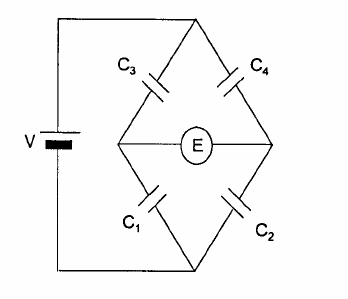
\includegraphics[width=5cm]{Selection_086.jpg} 
\end{figure}

Na ponte de capacitâncias da figura, o eletrômetro $E$ detecta a diferença de potencial entre os dois pontos entre os quais está ligado. Mostre que, quando a leitura de $E$ é zero, vale a relação

$$\displaystyle\dfrac{C1}{C2} = \displaystyle\dfrac{C3}{C4}$$

\textbf{RESOLUÇÃO}

\begin{figure}[h]	
\centering % para centralizarmos a figura	
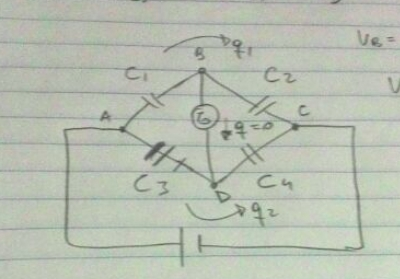
\includegraphics[width=5cm]{Selection_087.jpg} 
\end{figure}

Considerando que na figura acima os pontos $B$ e $D$ possuem o mesmo potencial, temos que para cada ramo do circuito passará uma quantidade de cargas $q_1$ e $q_2$ respectivamente. 

Calculando a diferença de potencial entre $A$ e $B$, temos:

\begin{equation}
V_a - V_b = \displaystyle\dfrac{q_1}{C_1}
\label{eq1}
\end{equation}

Calculando a diferença de potencial entre $A$ e $D$, temos:

\begin{equation}
V_a - V_d = \displaystyle\dfrac{q_2}{C_3}
\label{eq2}
\end{equation}

Como $V_b = V_d = 0$, e somando $\ref{eq1}$ e $\ref{eq2}$, ficamos:

\begin{equation}
\displaystyle\dfrac{q_1}{C_1} = \displaystyle\dfrac{q_2}{C_3}
\label{eq3}
\end{equation}

Calculando a diferença de potencial entre $B$ e $C$, temos:

\begin{equation}
V_b - V_c = \displaystyle\dfrac{q_1}{C_2}
\label{eq4}
\end{equation}

Calculando a diferença de potencial entre $D$ e $C$, temos:

\begin{equation}
V_d - V_c = \displaystyle\dfrac{q_1}{C_4}
\label{eq5}
\end{equation}

Como $V_b = V_d = 0$, e somando $\ref{eq4}$ e $\ref{eq5}$, ficamos:

\begin{equation}
\displaystyle\dfrac{q_1}{C_2} = \displaystyle\dfrac{q_2}{C_4}
\label{eq6}
\end{equation}

Dividindo $\ref{eq3}$ por $\ref{eq6}$, ficamos:

$$\displaystyle\dfrac{C_2}{C_1} = \displaystyle\dfrac{C_4}{C_3}$$

O que é válido com o que a questão pede.

\item \textbf{Griffiths - Cap.4 - Problema 4.25.}

O espaço entre as placas (de área A) de um capacitor plano está preenchido por duas camadas dielétricas adjacentes, de espessuras $d_1$ e $d_2$ e constantes dielétricas $k_1$ e $k_2$, respectivamente. A diferença de potencial entre as placas é $V$ e o campo aponta de 1 para 2. Encontre:

\begin{figure}[h]	
\centering % para centralizarmos a figura	
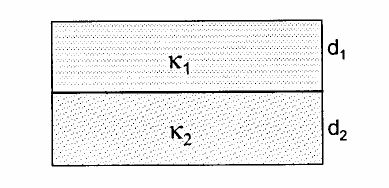
\includegraphics[width=5cm]{Selection_088.jpg} 
\end{figure}

\begin{enumerate}
\item A capacitância C do capacitor.
\item A densidade superficial de carga livre $\sigma$ nas placas.
\end{enumerate}

\textbf{RESOLUÇÃO}

\begin{enumerate}

\item

Pela lei de Gauss, o campo elétrico da placa de um capacitor plano é da seguinte forma:

$$E = \displaystyle\dfrac{Q}{\epsilon_0 A}$$

Se integrarmos esse campo para encontrarmos a diferença de potencial entre as placas do capacitor de $0$ a $d$, obtemos:

$$V = \displaystyle\dfrac{Qd}{\epsilon_0 A}$$

Aplicando esse resultado para achar a capacitância na relação $C = Q/V$, obtemos:

$$C = \displaystyle\dfrac{\epsilon_0 A}{d}$$

A capacitância de um dielétrico $C_{diel}$ depende de uma constante $\sigma$:

$$C_{diel} = \sigma C$$

$$C_{diel} = \sigma \displaystyle\dfrac{\epsilon_0 A}{d}$$

A capacitância total do capacitor é a soma da capacitância dos dois dielétricos:

$$C_1 + C_2 = \displaystyle\dfrac{\sigma_0\epsilon_0 A}{d_1} + \displaystyle\dfrac{\sigma_1\epsilon_0 A}{d_2}$$

Simplificando, obtemos:

$$\displaystyle\dfrac{1}{C} = \displaystyle\dfrac{d_1}{\sigma_0 \epsilon_0 A} + \displaystyle\dfrac{d_2}{\sigma_1 \epsilon_0 A}$$

\item

Pela relação geral para capacitores e considerando uma distribuição de cargas $Q = \sigma A$, temos:

$$Q = C V$$

$$\sigma A = C V$$

$$\sigma = \displaystyle\dfrac{CV}{A}$$



\end{enumerate}


\end{enumerate}
	
\end{document}